% -----------------------------------------------
% Template for SMAC SMC 2013
% adapted and corrected from the template for SMC 2012, which was adapted from that of SMC 2011
% further updated for TENOR 2015, 2016, 2017 and 2018
% -----------------------------------------------

\documentclass{article}
\usepackage{tenor}
\usepackage{ifpdf}
\usepackage[english]{babel}
\usepackage{balance}

\input{js-code-format}
\input{json-format}
%\usepackage{listings}


%%%%%%%%%%%%%%%%%%%%%%%% Some useful packages %%%%%%%%%%%%%%%%%%%%%%%%%%%%%%%
%%%%%%%%%%%%%%%%%%%%%%%% See related documentation %%%%%%%%%%%%%%%%%%%%%%%%%%
%\usepackage{amsmath} % popular packages from Am. Math. Soc. Please use the 
%\usepackage{amssymb} % related math environments (split, subequation, cases,
%\usepackage{amsfonts}% multline, etc.)
%\usepackage{bm}      % Bold Math package, defines the command \bf{}
%\usepackage{paralist}% extended list environments
%%subfig.sty is the modern replacement for subfigure.sty. However, subfig.sty 
%%requires and automatically loads caption.sty which overrides class handling 
%%of captions. To prevent this problem, preload caption.sty with caption=false 
%\usepackage[caption=false]{caption}
%\usepackage[font=footnotesize]{subfig}


% REDEFINE THESE VARIABLES:
\def\papertitle{Symbolist: bidirectional mapping developments}
\def\firstauthor{Rama Gottfried}
%\def\secondauthor{James Tsz-Him Cheung}
%\def\thirdauthor{Georg Hajdu}

\def\copyrightyear{2022}


\usepackage{xspace}
\def\symbolist{\textsc{symbolist}\xspace}
\def\drawsocket{\textsc{drawsocket}\xspace}
\def\uicontroller{\textit{ui\_controller}\xspace}
\def\iocontroller{\textit{io\_controller}\xspace}
\def\uiapiFunction{\textit{ui\_api}}
\def\uiapi{\textit{ui\_api}\xspace}
\def\ioapiFunction{\textit{io\_api}}
\def\ioapi{\textit{io\_api}\xspace}
\makeatletter
\newcommand{\verbatimfont}[1]{\renewcommand{\verbatim@font}{\ttfamily#1}}
\makeatother


%% Depending on the number of authors, set this variable accordingly for the copyright notice:
% \def\copyrightauthors{Author One}
\def\copyrightauthors{Rama Gottfried}
% \def\copyrightauthors{Author One, Author Two et al}

% adds the automatic
% Saves a lot of output space in PDF... after conversion with the distiller
% Delete if you cannot get PS fonts working on your system.

\def\oscfontsize{\footnotesize}


% pdf-tex settings: detect automatically if run by latex or pdflatex
\newif\ifpdf
\ifx\pdfoutput\relax
\else
   \ifcase\pdfoutput
      \pdffalse
   \else
      \pdftrue
\fi

\ifpdf % compiling with pdflatex
  \usepackage[pdftex,
    pdftitle={\papertitle},
    pdfauthor={\firstauthor},
    bookmarksnumbered, % use section numbers with bookmarks
    pdfstartview=XYZ % start with zoom=100% instead of full screen; 
                     % especially useful if working with a big screen :-)
   ]{hyperref}
  %\pdfcompresslevel=9

  \usepackage[pdftex]{graphicx}
  % declare the path(s) where your graphic files are and their extensions so 
  %you won't have to specify these with every instance of \includegraphics
  \graphicspath{{./figures/}}
  \DeclareGraphicsExtensions{.pdf,.jpeg,.png}

  \usepackage[figure,table]{hypcap}

\else % compiling with latex
  \usepackage[dvips,
    bookmarksnumbered, % use section numbers with bookmarks
    pdfstartview=XYZ % start with zoom=100% instead of full screen
  ]{hyperref}  % hyperrefs are active in the pdf file after conversion

  \usepackage[dvips]{epsfig,graphicx}
  % declare the path(s) where your graphic files are and their extensions so 
  %you won't have to specify these with every instance of \includegraphics
  \graphicspath{{./figures/}}
  \DeclareGraphicsExtensions{.eps}

  \usepackage[figure,table]{hypcap}
\fi

%setup the hyperref package - make the links black without a surrounding frame
\hypersetup{
    colorlinks,%
    citecolor=black,%
    filecolor=black,%
    linkcolor=black,%
    urlcolor=black
}


% Title.
% ------
\title{\papertitle}

\oneauthor
% \threeauthors
   {\firstauthor} { Hochschule für Music und Theater \\ Hamburg, Germany \\
     {\tt \href{mailto:rama.gottfried@hfmt-hamburg.de}{rama.gottfried@hfmt-hamburg.de}}}
% {\secondauthor} {University for Music and Theater \\ Hamburg, Germany  \\ 
%   {\tt \href{mailto:tsz.him.cheung@hfmt-hamburg.de}{tsz.him.cheung@hfmt-hamburg.de}}} 
% {\thirdauthor} {University for Music and Theater \\ Hamburg, Germany \\
%   {\tt \href{mailto:georg.hajdu@hfmt-hamburg.de}{georg.hajdu@hfmt-hamburg.de}}}



% ***************************************** the document starts here ***************
\begin{document}
%
\capstartfalse
\maketitle
\capstarttrue


% ABSTRACT
% fill in after finishing the paper
\begin{abstract}

maybe already start with history here, and then continue to symbolist?

  \symbolist is an in-development application for experimental notation, with the goal of creating a working environment for developing symbolic notation for multimedia which can be interpreted and performed by electronics. The program aims to provide an open play space, with tools for experimentation, and thinking visually about relationships between representation and interpretation in media performance. 
In the paper we discuss the evaluation and re-design of the application based on the need for a bi-directional mapping framework for working with symbolic notation and its corresponding data representations.

\end{abstract}


% INTRO
% not sure what should go here, or how in detail to go
% I guess:
% why did I make it, what is it, breifly discuss some of the steps

\section{Background}\label{sec:background}

The \symbolist project was developed out of an organic  

of compositional notation practice. 

how much of a background?

In this paper we present a case study for the creation of an open system for graphically developing symbolic notation which can function both as professional quality print or online documentation, as well as a computer performable score in electro-acoustic music and other computer aided contexts. Leveraging Adobe Illustrator’s graphic design tools and support for the Scalable Vector Graphics (SVG) file format~\footnote{https://www.w3.org/TR/SVG11/}, the study shows that SVG, being based on Extensible Markup Language (XML), can be similarly used as a tree-based container for score information. In the study, OpenSoundControl (OSC)~\cite{wright:osc}  serves as middleware used to interpret the SVG representation and finally realize this interpretation in the intended media context (electronic music, spatial audio, sound art, kinetic art, video, etc.). The paper discusses how this interpretive layer is made possible through the separation of visual representation from the act of rendering, and describes details of the current implementation, and outlines future developments for the project.

Initially developed as a method for performing vector graphics, 
SVG-OSC  \cite{gottfried2015svg}

\cite{maccallum2015dynamic} %middleware
%\cite{freed2014io} %io


XML nature of SVG makes it easy to parse and map just like and OSC bundle.

drawing on the OSC research at CNMAT, 

just like a piece of paper, SVG could be freely mappable, and \textit{performable} like OSC.



however it can require a lot of specialized code to handle different hierarchy structures and data at different levels in the hierarchy.


the first version of \symbolist was created as a standalone JUCE application
Ircam/ZKM~\cite{gottfried2018symbolist}

% this can probably be in the backstory part
\subsection{JUCE Version}\label{sec:juce_version}

explain juce version (include in overview?)
%\cite{krasner1988description}
focused on creating SVG and outputting OSC version (like SVG-OSC approach)


\subsection{Clefs and Bidirectional Mapping}\label{sec:bidirectional_mapping}

telling story of how we got where we are, conceptual steps

idea of Clefs

problem:
a lot of mapping is still needed

% drawsocket
\subsection{Drawsocket}\label{sec:drawsocket}

\cite{gottfried2019drawsocket}
\cite{hajdu2005quintet}



% Symbolist JS
\section{Symbolist JS}\label{sec:symbolist_js}

using \drawsocket as front end handler 


a general overview about need for classes (actually this comes later when we get into the the discussion of format i.e. the way the data is represented.

js and \drawsocket makes that easy(-ier)


Figure~\ref{fig:screenshot} shows a screenshot from the Electron version.


% screenshot
\begin{figure*}[ht!]
\centering
\includegraphics[width=2\columnwidth]{symbolist.png}
\caption{ \symbolist screenshot, showing some different types of staves, and editing capabilities.
\label{fig:screenshot}}
\end{figure*}


% Implementations
\section{Implementations}\label{sec:implementations}

Electron\footnote{https://www.electronjs.org/} version (node + chrome w/ special electron IPC)
Max version (node + jweb + Max patch for IPC)


\begin{figure*}[ht!]
\centering
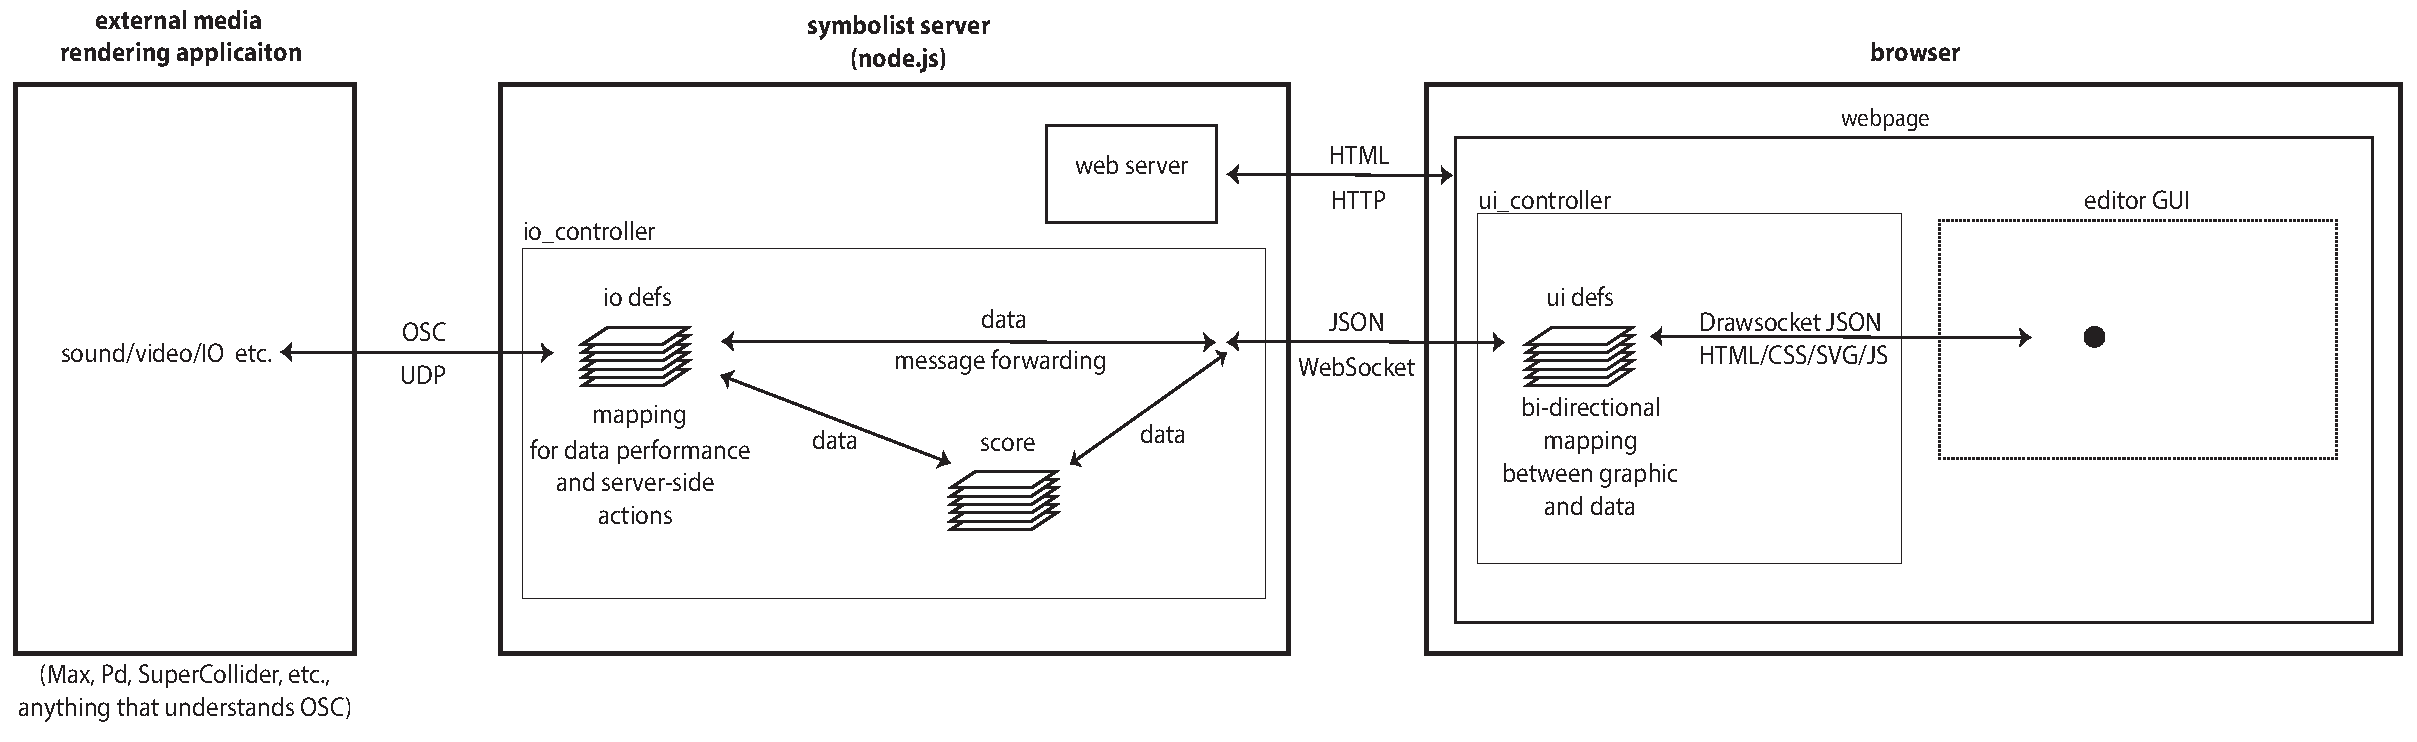
\includegraphics[width=2\columnwidth]{symbolist-architecture2.pdf}
\caption{ \symbolist architecture.
\label{fig:architecture}}
\end{figure*}

% Application Structure
\subsection{Application Structure}\label{sec:application_structure}

\symbolist is organized as a server-client model, comprising of:

\begin{enumerate}\itemsep0pt 
\item The \textit{editor}, a browser-based user interface client which displays the graphic representation of the data, and allows the user to edit and create new data objects through graphic interaction. The \uicontroller runs in the browser (see Figure~\ref{fig:architecture}), and handles interaction via a library of definition scripts which specify mappings to and from data and graphics formats, as well as other tools and interactions.

\item The \textit{symbolist server} runs in node.js (either in the context of Electron, or in Max's node.script object) and is comprised of: 
\begin{itemize}\itemsep0pt 

\item A HTTP web-server which serves the editor webpage, and manages messages between the \uicontroller and the \iocontroller via WebSocket connection, as well as handling operating system commands like reading and writing files.

\item  The \iocontroller script runs inside the \textit{symbolist server} and handles input and output from external sources via OSC over a UDP socket, and maintains the central \textit{score} database in its semantic data format (described below).
\end{itemize}
\end{enumerate}

%The \iocontroller holds a copy of the score in its semantic data format (described below), and loads a library of user scripts shared with the \uicontroller which define the mapping to (and potentially from) other media sources. 
%
%The \iocontroller can also be used to translate the score into other formats that can be performed by another sequencing tool or program like MaxMSP.
%

\section{Graphical Authoring and Interaction}\label{sec:editor} %should this be before or after the application structure?

%the palette symbol system is interesting maybe, to discuss how you can ``enter into'' a symbol, and then the possible sub-elements populate the palette.

The graphic user interface of \symbolist (Figure~\ref{fig:screenshot}) is designed around the idea of symbol objects and containers. Graphic objects, or \textit{symbols}, are placed in \textit{container} references which define a framing used to interpret the meaning of the \textit{symbol}.

In order to maintain an open and un-opinionated approach to authoring tools, \symbolist tries not to specify how containers and symbols should look, act, or respond when you interact with them within the application. 
Rather, the interaction and meanings of the symbols are defined in a library of custom object \textit{definitions} which create these meanings through mapping semantic data to and from the graphic visualization. 
Definitions can be shared between users and provide a mechanism to setup tailored composition environments for different authoring situations.

%See below for more information about the API for creating symbol definitions. 

\subsection{Interface Components}\label{sec:interface_components}

%main interesting thing to talk about is the palette system

Since the application is programmed using web-brower technologies (JS/HTML/CSS/SVG) there are many ways to customize the layout, using CSS, or defining new object types. 
The default \symbolist graphic editor (Figure~\ref{fig:screenshot}) provides the basic mechanisms for user interaction, to create scores through the creation of hierarchical object relationships.
The main graphic components are:

\begin{itemize}\itemsep0pt 
\item 
\textit{Document view}: the top level view of the application window, containing the document, and side bar. Sliders are provided to offset the view of the document, as well as basic zoom functionality.
\item 
\textit{Palette}: a set of buttons on in the side bar of the program which display icons of the \textit{symbols} that have been defined for the current selected \textit{container}. 
\item 
\textit{Tools}: a set of buttons that open tools for custom computer-assisted generation of new symbols, and applying transformations to existing elements (e.g. alignment of multiple objects, or setting distributing objects, etc.)
\item 
\textit{Inspector}: a contextual menu for editing the semantic data of an object, which is then mapped to the graphic representation.
\item 
\textit{Menu bar}: (Electron version only) the menu bar at the top of the screen or window, which provides access to various application functions.
\end{itemize}

\subsection{Modes}\label{sec:modes}

In the process of working in \symbolist, the user will shift between different modes, each of which have user-definable behaviors in the definitions library.
The current modes are:
\begin{itemize}\itemsep0pt 
\item \textit{Palette}: clicking on an icon in the palette sidebar enables the user interaction assigned to the clicked symbol type.
\item \textit{Creation}: holding down the CMD key (Mac) enters \textit{creation mode}, telling \symbolist to create a new \textit{symbol} of the type selected in the palette, similarly this action may enable different types of user interaction, for example snapping the symbol to specified pixels, etc.
\item \textit{Selection}: clicking on a pre-existing \textit{symbol} in the document will \textit{select} the object, which notifies a callback in the definition script for possible interaction.
\item \textit{Edit}: if a user has selected an object and then types the letter [e], \symbolist will attempt to enter \textit{edit mode} if there is one defined in the symbol definition script. This is useful for example in the case of a bezier curve; entering \textit{edit mode} could make visible the handles for the curve for editing.
\item \textit{Inspector}: if a user has selected an object and then types the letter [i], an inspector window appears showing the \textit{semantic data} corresponding to the symbol's graphical information (datatypes are discussed further in section~\ref{sec:representation} below).
\end{itemize}

% UX

\subsection{User Experience}\label{sec:ux}

On entering the application, the editor loads a score or configuration file from the default load folder, which sets the top-level page setup and palette options. A typical sequence of creating a score might be as follows:
\begin{enumerate}\itemsep0pt
\item The user opens a workspace, with one or more default \textit{container symbols} displayed on the screen, for example an empty rectangle which is like a piece of paper.
\item Selecting the ``paper'' container rectangle, the user then selects the container as the new \textit{context} by pressing the [s] key (or from the application menu).
\item Once setting the context, the palette toolbar is populated with icons of symbols that are defined with the selected container context type.
\item Clicking on one of the palette toolbar symbol icons, puts the interface into \textit{palette mode}, where the mouse interaction is now designed for use with this specific symbol type.
\item Holding the Mac CMD button enters \textit{creation mode} and by default creates a preview of the symbol how it will appear when you click, and some text is displayed near the mouse that shows the semantic data associated with the graphic representation.
\item After clicking the symbol is placed in the container.
\item Depending on the symbol type, you may be able to drag the symbol to a new place in the container, and the associated data is updated as a result.
\item Selecting the symbol and hitting the [i] button, brings up the inspector window, where you can edit the data and see the graphics updated in response.
\item Selecting and pressing the [e] button enters \textit{edit mode} which is a modal context where different user interaction could change the values of the symbol in different ways. For example in edit mode you might be able to rotate an object in a certain way, or be able to visualize different connections to the graphic representation to other elements of the score which are not usually highlighted in the score view.
\end{enumerate}


\section{Data Representation}\label{sec:representation}

At the heart of \symbolist are two parallel forms of information expression: \textit{semantic data} and \textit{graphic representation} (Figure~\ref{fig:graphic-representation}).

\textit{Semantic data} specifies the various attributes of information about a symbolic object, in terms of the object's meaning to the author. 
For example, the meaningful attributes of a \textit{note} object might be information about pitch and duration, or a \textit{point} object might contain x, y, and z values corresponding to the point's location in 3D space. In \symbolist \textit{semantic data} is thought of as the main holder of information in the system, which through grouping and hierarchical arrangement can be used to represent scores or other types of data structures.

The \textit{graphic representation} of the information is a visual expression of the semantic data, which is open in nature. The aim of \symbolist is to provide an agnostic framework for developing visual, symbolic, or other unknown representations of semantic data for use in multimedia composition practice; and so, one of the main functions of the new version of the software is to facilitate the creation of mapping relationships between different representations of the data.


\begin{figure}[ht!]
\centering
\includegraphics[width=1\columnwidth]{graphic-representation.pdf}
\caption{\textit{data} vs \textit{graphic} representation of the same information.
\label{fig:graphic-representation}}
\end{figure}



\section{Symbols}\label{sec:symbols}

In \symbolist terminology, a \textit{symbol} is an instance of a symbolic representation of data that connects the semantic, graphic, and possibly other media types of expression together as a multifaceted unit.
Each \textit{symbol} is defined as a \textit{class} of object, which specifies the symbol's data structure and UI interaction, and data mapping to different representational contexts.

\section{Semantic Data Format}\label{sec:format}

Within the \symbolist application, semantic data is stored as javascript objects, and read/written in JSON format~\footnote{https://www.json.org/json-en.html}, which is transcoded to and from OSC for inter-application communication.

The main attributes used in \symbolist semantic data objects are:

\begin{itemize}\itemsep0pt 
\item \textit{id}: a unique identifier name (required).
\item \textit{class}: a reference to the definition of the object type in the user-definition library (required).
\item \textit{contents}: an array of child objects that a parent container object might hold (required for container symbols).
\end{itemize}

In addition to the required \textit{id} and \textit{class} attributes, symbol objects may include any number of other \textit{attributes}\footnote{The term \textit{attribute} is used here interchangeably with properties, parameters, aspects, etc.} of the symbol (\textit{pitch}, \textit{amplitude}, etc.). For example a simple semantic object written in JSON might look like:

\begin{lstlisting}[
  mathescape,
  columns=fullflexible,
  breaklines=true,
  basicstyle=\oscfontsize\fontfamily{lmvtt}\selectfont,
]
{
    "id" : "foo",
    "class" : "legs",
    "action" : "jump",
    "start_time" : 0.1
}
\end{lstlisting}

\noindent
Here we see an object with the \textit{id} ``foo,'' which is of \textit{class} type ``legs'', that has an attribute \textit{action} associated with it and a start time.

\subsection{Containers}
Symbols may also contain other symbols. 
Container symbols function to frame their contents, giving reference and context, like a plot graph frame, which provides a perspective and scaling for interpreting the set of data points displayed in the graph.

When a symbol contains other symbols, the child symbols are stored as an array in the object's \textit{contents} field. For example an imaginary class ``timeline'', which holds two types of leg actions, we might write something like:

\begin{lstlisting}[
  mathescape,
  columns=fullflexible,
  breaklines=true,
  basicstyle=\oscfontsize\fontfamily{lmvtt}\selectfont,
]
{
    "id" : "bar",
    "class" : "timeline",
    "duration" : 1,
    "contents" : [{
        "id" : "foo-1",
        "class" : "legs",
        "action" : "jump",
        "start_time" : 0.1
    },{
        "id" : "foo-2",
        "class" : "legs",
        "action" : "sit",
        "start_time" : 0.2
    }]
}

\end{lstlisting}

% move this to the definitions discussion?
In most cases, a symbol's mapping definition will require querying its parent symbol for information, in order to plot its data relative to the container context, for example offsetting the screen coordinate position based on the parent object position.

\section{Score File Format}\label{sec:score}

Using symbols and symbol containers, we can create tree structures which can be used to represent hierarchical grouping; to represent scores, or other types of data structures.
At the root of the tree structure is a top-level symbol, which might (but not necessarily) define behavior of its children objects.
Since the data elements are stored in js objects, it is easy to import/export \symbolist scores as JSON files.

When the application loads, it reads a default initialization file, in the form of a \symbolist score.
The current default initialization config file looks like this:

\begin{minipage}{\linewidth}
\begin{lstlisting}[
  mathescape,
  columns=fullflexible,
  breaklines=true,
  basicstyle=\oscfontsize\fontfamily{lmvtt}\selectfont,
]
{
    "about" : "symbolist will read a json file to configure the palette setup, this can be used to dynamically change the application layout and tools",
    "id" : "Score",
    "class" : "RootSymbol",
    "tools" : [],
    "palette" : ["SubdivisionTool", "BasicSymbolGL"],
    "contents": { 
        "id" : "trio",
        "class" : "SystemContainer",
        "x": 200,
        "y": 100,
        "duration": 20,
        "time": 0,
        "contents" : [{
            "id" : "oboe",
            "class" : "FiveLineStave",
            "height" : 100,
            "lineSpacing" : 10,
            "duration": 20,
            "time": 0,
            "contents" : []
        },
        {
            "id" : "bassoon",
            "class" : "PartStave",
            "height" : 100,
            "time": 0,
            "duration": 20,
            "contents" : []
        },
        {
            "id" : "synth",
            "class" : "PartStave",
            "height" : 200,
            "time": 0,
            "duration": 20,
            "contents" : []
        }]
    }
}
\end{lstlisting}
\end{minipage}

The initialization file is literally a score object file, providing the default context for a given authoring situation. In this example, we can see there is a ``RootSymbol'', which contains a ``SystemContainer'', which in turn contains two ``PartStave'' symbols and one ``FiveLineStave'' symbol (which are all actually containers as well, initialized as empty arrays). The \textit{palette} and \textit{tools} attributes tell the application to provide access to certain tools, and child symbols in the GUI.

\section{Graphic Display Format}\label{graphic_display_format}

The graphic representation of the data in \symbolist uses SVG format, and and follows the same hierarchical structure of the data as found in the semantic data score object.
Since the new version of \symbolist uses a browser as a frontend, we are able to take advantage of the many standard tools and web functionalities provided by browsers for display, interaction and data management.

Like the JSON score initialization file above, the main application window is setup using HTML/CSS, and utilizing \drawsocket as a convenience wrapper to provide shorthand methods to create and manipulating browser window elements. 

\subsection{SVG}

The \symbolist format for an SVG \textit{symbol} is a one top group ($<$g$>$) elements, with two sub-groups for \textit{display} and \textit{contents}, using HTML/CSS class names. The most simple SVG symbol would be:

\begin{lstlisting}[mathescape, columns=fullflexible, breaklines=true,basicstyle=\oscfontsize\fontfamily{lmvtt}\selectfont]
<g  id="foo" class="SymbolClassName symbol">
    <g class="SymbolClassName display"></g>
    <g class="SymbolClassName contents"></g>
</g>
\end{lstlisting}


Just like the semantic data objects, graphics objects have required \textit{id} and \textit{class} parameters, with an optional \textit{contents} element.

Each symbol grouping element is tagged using class names, following the symbol's unique class name (in this example ``SymbolClassName''). Note that the order is important: \textit{the symbol class type must be first}. The \textit{symbol} tag marks the top-level grouping object of the symbol, the \textit{display} element is a group that holds all of this symbol's visual display information, and the \textit{contents} is an group object for holding any potential child elements. Note that for simplicity, all \symbolist graphic elements include the \textit{contents} element as a placeholder.

\subsection{HTML}

Symbols and containers could also potentially be HTML elements instead of SVG. In the case of HTML you would use $<$div$>$ tags instead of SVG $<$g$>$:
html:

\begin{lstlisting}[
  mathescape,
  columns=fullflexible,
  basicstyle=\oscfontsize\fontfamily{lmvtt}\selectfont,
]
<div class="SymbolClassName symbol">
    <div class="SymbolClassName display"></div>
    <div class="SymbolClassName contents"></div>
</div>
\end{lstlisting}


\subsection{dataset-elements}\label{sec:dataset}

Since \symbolist is constantly mapping to and from semantic data and its graphic representation, we are using the HTML \textit{dataset} feature\footnote{https://developer.mozilla.org/en-US/docs/Web/API/HTMLElement/dataset} to store the semantic data inside the top-level \textit{symbol} element ($<$g$>$ or $<$div$>$).
The HTML dataset attributes use the prefix ``\textit{data-}''.\footnote{Note that according to the HTML dataset specifications, all names will be converted to lowercase, this can create issues in some cases, so best practice is to use all lowercase for attribute names.}

For example, mapping our imaginary ``legs'' actions above, the corresponding SVG objects would be (skipping the actual display drawing for now):

\begin{minipage}{\linewidth}
\begin{lstlisting}[
%float=*,
mathescape, columns=fullflexible, breaklines=true,basicstyle=\oscfontsize\fontfamily{lmvtt}\selectfont]
<g  id="bar" class="Timeline symbol" data-duration="1">
  <g class='Timeline display'></g>
  <g class='Timeline contents'>
      <g  id="foo-1" class="Legs symbol" data-action="jump" data-start_time="0.1">
        <g class='Legs display'></g>
        <g class='Legs contents'></g>
      </g>
      <g  id="foo-2" class="Legs symbol" data-action="sit" data-start_time="0.2">
        <g class='Legs display'></g>
        <g class='Legs contents'></g>
      </g>
    </g>
</g>
\end{lstlisting}
\end{minipage}




\section{Performing Data}

Just as the \textit{graphic representation} can be seen as a visual expression of \textit{semantic data}, the same semantic data can also used as control data in connection with other media forms. For example, a \textit{note} object's pitch, onset, and duration information could be used to trigger a note on a synthesizer, or a sequence of Labanotation~\cite{guest2014labanotation} could be used to guide the movement of robotic motors, create haptic feedback for live performance~\cite{west2019design}, and so on. 

\symbolist provides several different options for sorting and looking up data (see Figure~\ref{fig:score-lookup}), which can serve as a structure for the performance of a ``score'', or other data formats. Typically, some representation of time is used to indicate an object's moment of action, but in \symbolist the exact nature of the temporal organization is up to to the author (see section \ref{subsec:io_messages} for further discussion of performing data). 

In addition to the \textit{semantic} and \textit{graphic} contexts of data representation, we can think of the \textit{performance} of the data as a third data context context.

\section{Mapping}\label{sec:mapping}

Between each of these representation contexts there is a layer of mapping, with the \textit{semantic data} serving as the primary representation type. 

\textit{Semantic data to graphic representation} mapping (Figure~\ref{fig:data-to-graphic}) is used for the creation of graphic symbols from a stream of input, for example from generative processes, textural authoring, or computer assisted composition systems~\cite{bresson2011om, didkovsky2008maxscore, agostini2015max, baca2015abjad, burloiu2017visual}.

\textit{Graphic representation to semantic data} mapping (Figure~\ref{fig:graphic-to-data}) is used in order to create or edit data based on graphic information. This is the typical ``graphical user interface'' situation, where the data is accessible through its visual representation.

\textit{Semantic data to performance media} mapping (Figure~\ref{fig:score-lookup}) is the use of the data as a sequence of events that can be played in time (or used to control other processes not necessarily in time).

Note that in \symbolist mapping between \textit{performance media} and \textit{graphic representation} is achieved through first mapping to semantic data. See section~\ref{library_definitions_api} for further discussion.


% mapping figures

\begin{figure}[ht!]
\centering
\includegraphics[width=0.9\columnwidth]{data-to-graphic.pdf}
\caption{\textit{semantic data} mapped to create a \textit{graphic} representation from input data.
\label{fig:data-to-graphic}}
\end{figure}

\begin{figure}[ht!]
\centering
\includegraphics[width=0.9\columnwidth]{graphic-to-data.pdf}
\caption{If edited graphically, the updated graphic data is then mapped back to \textit{semantic data} representation. 
\label{fig:graphic-to-data}}
\end{figure}

\begin{figure}[ht!]
\centering
\includegraphics[width=1\columnwidth]{score-lookup.pdf}
\caption{Using the lookup method defined by the symbol class, the \textit{semantic data} can be used to perform external instruments via Open Sound Control. 
\label{fig:score-lookup}}
\end{figure}

\section{Symbol Definitions}\label{library_definitions_api}
%Definition scripts are composed as Javascript modules which are loaded into the program at runtime.

Symbols are defined as Javascript classes which are stored and recalled when symbol actions are performed. 
Through creating definitions, users are able to form libraries of symbols that can be used together to fit the tools and representation to address a given use-case scenario.
Definitions define the mapping relationships between the symbol's \textit{semantic}, \textit{graphic}, and output \textit{performance} data.
%Definitions allow for custom graphical user interaction for each type of symbol, and are used to define mapping relationships between the symbol's \textit{semantic}, \textit{graphic}, and output \textit{performance} data.

To allow for maximum flexibility of interaction and the creation of context-specific composition environments, each symbol manages its own mouse interaction, triggered by the user's selection in the palette toolbar. 
In order to streamline the process of writing new symbol definitions there is a template base class that handles most common interaction situations, which can be redefined and overwritten by sub-classes. Eventually it is planned to provide a UI in the editor for defining a mapping definition graphically, but this is not yet implemented.

There are two types of definition scripts:
\begin{itemize}\itemsep0pt 
\item \textit{ui-definitions} run in the \uicontroller and perform user interactions based on the different interaction modes described above, and apply bidirectional mapping between semantic data representation and graphic representation in the browser.
\item \textit{io-definitions} run in the \iocontroller and are used to assist in the lookup and \textit{performance} mappings of the semantic data to media like sound synthesis, video, etc., or to perform server-side score manipulations.
\end{itemize}

In each controller context there are certain methods and variables that need to be defined in order for the class to function properly in the \symbolist ecosystem.

%Currently, the system uses the same .js file to hold both the `ui` and `io` definitions. To aid in development there is a template file that can be used to handle most of the most common actions.

\subsection*{IO and UI data access scope}\label{sec:io_ui_elements}

Since the \textit{ui} and \textit{io} controllers are run in separate processes\footnote{and potentially separate devices.} (Figure~\ref{fig:architecture}), there is no direct access to data stored in the other location. In other words, the \iocontroller does not have direct access to the symbol's drawing information, and the \uicontroller does not have direct access to the score or UDP port for sending OSC message.

Loosely following the MVC pattern,\footnote{https://developer.mozilla.org/en-US/docs/Glossary/MVC} the concerns of drawing are kept within the browser-side \uicontroller, with all messages between the \textit{ui} and \textit{io} processes are in \drawsocket JSON format, with all symbol data expressed in its \textit{semantic} form.
Meanwhile the \iocontroller manages the \textit{score} and handles external OSC communication, relaying messages to the \uicontroller as needed.

As discussed above, the graphic representation takes advantage of the HTML dataset feature, which provides a mechanism for storing the semantic data inside the graphic context (see section~\ref{sec:dataset}).
Since ui-definitions are running in a web-browser, they are able to make use of the standard HTML-DOM JS methods for fast querying of elements (i.e. querySelector, getElementById, etc.)\footnote{https://developer.mozilla.org/en-US/docs/Web/API/Document} to retrieve graphic as well as semantic data stored in the display hierarchy.

To provide similar data query access in the \iocontroller, the score data is stored in two JS objects: the \textit{score}, which stores the semantic data in a hierarchical tree structure, and a object named \textit{model}, which is a flat lookup table by unique id, with links to object references to the coordinated object in the score tree.

Since the ui- and io-controllers run in parallel they need to keep the other side updated in case of any alteration to the score data. 
Updates sent from the \iocontroller to the UI can be as simple as sending a new score which will trigger a redrawing of the graphics in the UI view. 
Updates from graphic user interaction require mapping from the graphic to semantic representation, which is handled in the browser. Any changes are sent back to the \iocontroller where the new semantic values are updated in the \textit{model} (which automatically update the \textit{score}, since both objects hold JS references to the same JS objects).

\subsection*{API Functions}\label{sec:api_functions}

In each controller context, there are a set of helper functions for use by symbol definitions stored in global objects called \uiapi and \ioapi, which provide many essential operations.

\subsection{UI Definitions}\label{sec:ui_callbacks}

Variables and methods called by the \uicontroller are:

\begin{itemize}\itemsep0pt 
\item \textit{class}: the unique name of the symbol.
\item \textit{palette}: used for container symbols, an array of class names of other symbols that can be used within this container.

\item \textit{getPaletteIcon}: called when drawing the palette for a given container; returns an icon for display in the palette toolbar, using \drawsocket format.

\item \textit{paletteSelected}: called when the user clicks on the palette icon for this symbol, used to trigger custom UI. When the symbol is selected in the palette, the definition should enable its mouse handers. For creating new symbols from mouse data (currently \textit{cmd-click} is the convention).

\item \textit{getInfoDisplay}: called when creating the inspector window; returns drawing commands for the inspector contextual menu, for convenience \uiapi provides a function called \textit{makeDefaultInfoDisplay} which can be used in most cases.

\item \textit{fromData}: called when data is should be mapped to graphic representation. The definition is responsible for creating the graphic element, normally via \drawsocket, but other approaches are also possible.

\item \textit{updateFromDataset}: called from the inspector when elements of the data should be updated. Usually this function will call \textit{fromData} to redraw the graphic symbol, and should also send the updated data to the server.

\item \textit{selected}: called on selection and deselection, return true if selection is handled in the script, returning false (or no return) will trigger the default selection mechanics by the \uicontroller.

\item \textit{drag}: called from \uicontroller when the user drags selected symbols. For best results, the use the \uiapi \textit{translate} function to set the symbol's SVG translation matrix, but do not apply the translation until mouse up to avoid incremental state changes to score.

\item \textit{applyTransformToData}: called on mouse-up if selected objects have changed. Definition should then apply the transform matrix to the SVG attribute values. This is important because the attribute values not the translation matrix are used for mapping. The \uiapi helper function \textit{.applyTransform} is provided for convenience.

\item \textit{currentContext}: called when the user enters or exits a container symbol (hitting the [s] key, [esc] to exit).

\item \textit{editMode}: called when entering and exiting edit mode.
\end{itemize}

\subsubsection{Data and View Parameters}

Probably the most important elements of the symbol definition is the bi-directional mapping between semantic and graphic forms. 
Looking at Figures~\ref{fig:data-to-graphic} and \ref{fig:graphic-to-data} we can see that in some cases the relationship between a semantic property and its graphic representation is not a one-to-one mapping.
For instance in Figure~\ref{fig:data-to-graphic} the \textit{note} property needs to be mapped to a pixel position that is used for both the center point of a graphic circle (note-head) as well as the starting point for a line (duration indication).
In reverse, Figure~\ref{fig:graphic-to-data} shows how when the user moves a symbol graphically, the new pixel positions need to be translated back into semantic data in order to update the score.
This can get somewhat complex in cases of nonlinear mappings, and one-to-many data to graphic situations.

In order to manage the mapping between semantic and display representation, the template base class uses an intermediate mapping stage called \textit{view-parameters}.
The idea is that the \textit{view-parameter} stage contains the bare-minimum number of variables needed to draw the symbol.
For example, in Figure~\ref{fig:data-to-graphic} the graphic representation requires a \textit{y} position relative to the pitch, an \textit{x} position relative to the start time, and a \textit{width} value relative to the duration of the event (the amplitude is not displayed).
After first mapping from the semantic attributes \textit{note}, \textit{start-time} and \textit{duration} to view-parameters \textit{x}, \textit{y}, and \textit{width}, the drawing method can then use the \textit{x}, \textit{y}, and \textit{width} values to draw its two graphic objects from the reduced set of view-parameters values.

The ui template class uses two functions to define data-view mappings: \textit{dataToViewParams} which receives the semantic data object and returns the view-parameter object, and \textit{viewParamsToData} which performs the opposite mapping.
Note that in many cases the \textit{viewParamsToData} function needs only one aspect of the graphic to map back to semantic data. In the example shown in Figure~\ref{fig:graphic-to-data}, the mapping only really needs either the center point of the note-head or the start-x position of the line to determine the \textit{start-time} parameter.

The template class also two additional data/view-parameter methods to coordinate child objects with parent containers: \textit{childDataToViewParams} and \textit{childViewParamsToData}.
For example, in Figures~\ref{fig:data-to-graphic} a note-head circle is drawn from its \textit{note} parameter, in coordination with a five-line staff.
Like a plot graph, the \textit{staff} is a container symbol which defines how we interpret the elements written on its lines. 
In this case, the symbol definition for the \textit{staff} has a \textit{childDataToViewParams} function is called by the action of the child symbol. 
The \textit{childDataToViewParams} receives the child data object, as well as the graphic element of a particular staff (which was selected by the user pressing the [s] key). Given its placement on the screen and its own data parameters (number of lines, clef, etc.) the staff's \textit{childDataToViewParams} function will return the view parameters for the child, mapped in relationship to the container object.
Similarly, when the graphic object is moved, the child object will call the parent's \textit{childViewParamsToData} function to assist with mapping back to semantic data format.


\subsection{IO Definitions}\label{sec:io_messages}

Variables and methods called by the \iocontroller are:

\begin{itemize}\itemsep0pt 
\item \textit{class}: class name, corresponding to class name in UI Definition.

\item \textit{comparator}: comparator function used in container symbols to sort child symbol. For example, if a given container uses a \textit{time} value for sorting, when a new child node is added, the comparator function helps the container insert the child element at the correct location in the \textit{contents} array.

\item \textit{lookup}: called via OSC (using the \drawsocket syntax \textit{key} ``lookup'') to look up events at a given value specified by the container (e.g. typically \textit{time}). The \textit{lookup} function performs hit detection collecting all active elements at that query point, output back to the calling application via OSC (the in/out UDP port information is set in the \symbolist configuration file). By default the output is an array of all active data objects at the lookup point, along with the relative phase position within each element, useful for controlling amplitude envelopes etc. (See Figure~\ref{fig:score-lookup}).

\item \textit{getFormattedLookup}: called via OSC to request a complete list of events for external sequencing, formatted in the symbol definition to apply to the external syntax requirements.
%For example, this function might return a list of \textit{/x} and \textit{/y} values for use with the \textit{o.lookup$\sim$} Max object, or create a MIDI file export etc.
% references for o.lookup? or maybe take this out, too specific

\end{itemize}

Note that all parameters included in the input \drawsocket syntax \textit{val} object will be included in the data received by \textit{lookup} and \textit{getFormattedLookup} as a parameters, and can then be used when performing the lookup, for example to perform multidimensional nearest neighbor lookup, etc.

\subsection{Custom User Methods}\label{sec:call}

Users may also create their own methods in either ui or io-definitions and call them from outside processes over OSC, using the ``call'' keyword.
\symbolist will pass the same call request to both definitions, so if both have a function of the same name they will both be called. 
%Return values from the \textit{io} controller are with the tag \textit{return/io} and \textit{return/ui} from the \textit{ui}.

Required parameters:

\begin{itemize}\itemsep0pt 
 \item \textit{class}: name of the class to lookup.
  \item \textit{method} name of class method to call.
\end{itemize}

All of the parameters in the \textit{val} object will be passed to the function as an argument. 

User class methods can be used to apply operations to the score or ui, for example transposing all pitches on the ``Staff'' named ``oboe'' might look like this:

\begin{lstlisting}[
  mathescape,
  columns=fullflexible,
  basicstyle=\oscfontsize\fontfamily{lmvtt}\selectfont,
]
{
    /key : "call",
    /val : {
        /class : "Staff",
        /method : "transpose",
        /id : "oboe"
        /steps : 12
    }
}
\end{lstlisting}

The implementation in the io definition could then lookup the class ``Staff'' and call the method ``transpose'', passing the entire \textit{val} object to the function as an argument. The ``transpose'' function would then lookup the ``oboe'' staff in the model, and then iterate all of its contents, offsetting the ``note'' values by the number of steps specified in the method arguments.

\section{Symbol Definition Functional Examples}

\subsection{Creating Symbols from OSC input}

The simplest example of mapping definition is the \textit{semantic to graphic} mapping definition.

\subsubsection{OSC is received by the \iocontroller}

The \iocontroller has a set of messages that it understands which can be used for a wide range of actions.
\symbolist uses the \drawsocket \textit{key/val} message syntax, so each OSC bundle should be formatted with a \textit{key} address, which is a keyword flag to signal which routine should interpret the message in the \iocontroller's \textit{io\_receive} function; while the \textit{val} address contains an object (or array of objects) to be processed.

And OSC message with the \textit{data} keyword can be used to add new semantic data objects to the score-model, and create new graphic symbols in the editor from an external process;  for example by generating scores through algorithmic processes, via textual authoring, via mapping from gestural controller, etc.

Upon receiving an OSC message with a \textit{data} flag, the object attached to the \textit{val} address are added to the model, and then relayed to the \uicontroller.
In the \uicontroller, the semantic data is mapped to graphic data using the symbol's \textit{class} definition. The class's name provides a mechanism to lookup the class definition in both controller scripts.

For example, here is an OSC bundle using the \textit{data} key:

\begin{lstlisting}[ mathescape, columns=fullflexible, basicstyle=\oscfontsize\fontfamily{lmvtt}\selectfont ]
{
    /key : "data",
    /val : {
        /class : "FiveLineStaveEvent",
        /id : "foo"
        /container : "oboe",
        /time : 0.13622,
        /ratio : "7/4",
        /duration : 0.1,
        /amp : 1
    }
  }
\end{lstlisting}

The \textit{data} key has a few required and optional attributes:
\begin{itemize}\itemsep0pt 
  \item \textit{class}: (required) the class type of the object to create.
  \item \textit{container}: (required) the \textit{id} of the container symbol class to put the object in.
   \item \textit{id}: (optional) an id to use for the data object, if non is specified a (long) unique string will be generated.
  \item Other required or optional parameters will depend on the symbol definition.
\end{itemize}

% this is the second part of the process:

\subsubsection{Data to View Mapping in the \uicontroller}

fromData

If an OSC message is received containing data to create a new symbol, the \uicontroller calls the object's `fromData` function, which maps from the data representation to the graphic drawing commands. The `fromData` function should:
1. send the drawing commands to the browser display (via \drawsocket usually, using the `drawsocketInput` API method). Include the data content into the symbol by using the HTML `dataset` (you can use `ui\_api.dataToHTML(dataObj)` helper function to create the `data-` tags)

\begin{lstlisting}[ language=Javascript]
    ui_api.drawsocketInput({
        key: "svg",
        val: {
            class: `${className} symbol`,
            id: uniqueID,
            parent: container.id,
            ...newView, 
            ...ui_api.dataToHTML(dataObj)
        }
    }) 
\end{lstlisting}


\subsection{Creating Data from Graphic Interaction}

briefly describe the sequences of events
 

createNewFromMouseEvent (template function)

Working from the opposite direction, users can create semantic data entries in the score through graphic interaction. The process for achieving this is a bit more complicated than the 


%%%%%

\section{temp}

%%
\symbolist has built in handlers for a set of messages received via OSC, which can be extended by user scripts, using a key/val syntax, where the \textit{key} specifies the function to call, and the \textit{val} are the parameter values to use for the call.

For example, here is a \textit{lookup} query to find elements that are returned by the parameters \textit{time} in the container with the \textit{id} ``trio''.


\begin{lstlisting}[
  mathescape,
  columns=fullflexible,
  basicstyle=\oscfontsize\fontfamily{lmvtt}\selectfont,
]
{
    /key : "lookup",
    /val : {
        /time : 0.1,
        /id : "trio"
    }
}

\end{lstlisting}

The OSC message API supports the following keys:
\begin{itemize}\itemsep0pt 
\item \textit{data}: adds a data object to the score, and sends to the ui to be mapped to graphical representation. Parameters include:
\begin{itemize}\itemsep0pt 
  \item \textit{class} (required) the class type of the object to create
  \item \textit{container} (required) the container symbol class to put the object in (in case there are multiple containers that support the same symbol type)
  \item \textit{id} (optional) an id to use for the data object, if non is specified a (long) unique string will be generated.
  \item Other required or optional parameters will depend on the symbol definition.
\end{itemize}

\begin{lstlisting}[ mathescape, columns=fullflexible, basicstyle=\oscfontsize\fontfamily{lmvtt}\selectfont ]
{
    /key : "data",
    /val : {
        /class : "fiveLineStaveEvent",
        /id : "foo"
        /container : "oboe",
        /time : 0.13622,
        /ratio : "7/4",
        /duration : 0.1,
        /amp : 1
    }
  }
\end{lstlisting}


\item \textit{lookup}: looks up a point in a container, based on a sorting function specified in the definition. For example, this can be used to get all events active at a given time. Parameters:

\begin{itemize}\itemsep0pt 
  \item \textit{id}: (required) the \textit{id} of the container to lookup in. Containers will generally iterate all child objects, so for example if you use the \textit{id} of the top level score you should be looking up in to all sub-containers.
  \end{itemize}
  
\item \textit{getFormattedLookup}: optional function that might be defined in an \textit{io} script that outputs an object formatted for a different type of player/render. For example, this function might return a list of \textit{/x} and \textit{/y} values for use with the \textit{o.lookup~} Max object, or create a MIDI file export etc. All parameters included in the \textit{val} object will be sent to the \textit{getFormattedLookup} as a parameters object. Parameters:

\begin{itemize}\itemsep0pt 
  \item \textit{id}: (required)
\end{itemize}
\item \textit{call}: calls a function in the one or both of the class definitions. All of the parameters in the \textit{val} object will be passed to the function as an argument. Return values from the \textit{io} controller are with the tag \textit{return/io} and \textit{return/ui} from the \textit{ui}.
\begin{itemize}\itemsep0pt 
  \item \textit{class} (required) class of the object to call
  \item \textit{method} (required) name of object function to call
\end{itemize}

\end{itemize}

\begin{lstlisting}[
  mathescape,
  columns=fullflexible,
  basicstyle=\oscfontsize\fontfamily{lmvtt}\selectfont,
]
{
    /key : "call",
    /val : {
        /function : "functionName",
        /class : "className",
        /id : "foo"
        /someValue : 1,
        /anotherValue : 2
    }
}
\end{lstlisting}

Note that the system will pass the same call to both definitions, so if both have a function of the same name they will both be called.
* \textit{drawsocket}: forwards \drawsocket format messages directly to \drawsocket, bypassing the symbolist mapping.


% screenshot
\begin{figure*}[ht!]
\centering
\includegraphics[width=1.5\columnwidth]{nodescore.png}
\caption{ \symbolist screenshot, showing some different types of staves, and editing capabilities.
\label{fig:nodescore}}
\end{figure*}

\section{Conclusions and Future Developments}

known issues
- unable to dynamically refresh definitions in the browser using the require function after Electron v12, using Context Isolation\footnote{https://www.electronjs.org/docs/latest/tutorial/context-isolation} as suggested to address possible security issues, currently webpack is used to bundle the definitions
>> need to look into what is possible, since for user defined scripts we definitely will want to be able to tweak them without running webpack again.

continue work on CP notation
GUI for definitions
C/C++ score player, optimized for fast lookup - write to buffer?
further experiments in representation, spatial audio, eurorack modules, 
connect with antescofo?
connect with faust? create audio code via faust, or maybe pd?
networked display via \drawsocket compose on tablets with pen?

\begin{acknowledgments}
thanks james! thanks georg! thanks jean!
\end{acknowledgments} 

%%%%%%%%%%%%%%%%%%%%%%%%%%%%%%%%%%%%%%%%%%%%%%%%%%%%%%%%%%%%%%%%%%%%%%%%%%%%%
%bibliography 
\balance % balance the columns on the last page
\bibliography{symbolist}
\end{document}
